\documentclass[nofonts, oneside]{ctexbook}

\usepackage{xeCJK}
\usepackage{hyperref}
\usepackage{makeidx}
\usepackage{listings}
\usepackage{geometry}

\newcommand\shellcmd[1]{\texttt{#1}}
\newcommand\svn{\texttt{svn}}
\newcommand\svnci{\texttt{commit}}
\newcommand\svnco{\texttt{checkout}}
\newcommand\svnlog{\texttt{log}}
\newcommand\svnst{\texttt{status}}
\newcommand\svndf{\texttt{diff}}
\newcommand\svnup{\texttt{update}}
\newcommand\svngcc{\texttt{gcc}}
\newcommand\svnrv{\texttt{revert}}
\newcommand\svnpwd{\texttt{pwd}}
\newcommand\svnmg{\texttt{merge}}
\newcommand\svncat{\texttt{cat}}
\newcommand\svnadd{\texttt{add}}
\newcommand\svnrs{\texttt{resolve}}
\newcommand\svncp{\texttt{copy}}
\newcommand\svnls{\texttt{ls}}

\hypersetup {
    bookmarksnumbered = true,
    pdfborder = 0 0 0
}

\lstnewenvironment{svnshell}
  {
    \lstset{basicstyle = \ttfamily,
        tabsize = 4,
        frame = single,
        escapechar = &,
        breaklines = true,
        breakatwhitespace = true,
    }
  }
  {}
\lstnewenvironment{ccode}
  {
    \lstset{basicstyle = \ttfamily,
        tabsize = 4,
        frame = single,
        escapechar = `,
        breaklines = true,
        breakatwhitespace = true,
    }
  }
  {}

\makeindex
\setCJKmainfont{AR PL KaitiM GB}
\setCJKsansfont{WenQuanYi Zen Hei}
\setCJKmonofont[Scale=0.9]{WenQuanYi Zen Hei}
\setmainfont{Century Schoolbook L}
\setsansfont{FreeSans}
% "Mapping={}" make quote symbol straight
\setmonofont[Mapping={}]{Courier 10 Pitch}

\geometry{%
    top = 2.5cm,
    bottom = 2cm,
    outer = 2.5cm,
    inner = 2.5cm
}

\title{SVN 教程}
\author{\url{www.tutorialspoint.com/svn/index.htm} \and
	\url{https://github.com/wuzhouhui/svn}}

\begin{document}

\maketitle

\chapter{基本概念}
\label{chap:basic_concepts}

\section{什么是版本控制系统}
\label{sec:what_is_version_control_system}

版本控制系统 (Version Control System, 简称 VCS) 是一种软件, 它可以帮助软件开
发人员协同工作, 以及管理产品的完整历史.

版本控制系统的目标包括:
\begin{itemize}
  \item 支持多人同时操作.
  \item 不覆盖其他人作出的修改.
  \item 维护每一个版本的历史.
\end{itemize}

VCS 可以分成两大类别:
\begin{itemize}
  \item 集中式的版本控制系统 (Centralized Version Control System, 简称 CVCS);
  \item 分布式的版本控制系统 (Distributed Version Control System, 简称 DVCS).
\end{itemize}

本教程只讨论 CVCS, 特别是 Subversion, 它使用中央服务器来存
储所有的文件, 并支持团队协作.

\section{版本控制术语}
\label{sec:version_control_terminologies}

首先先来介绍本教程将会用到的几个术语.

\begin{itemize}
  \item 仓库 (Repository): 仓库是所有版本控制系统的
      核心, 它是开发人员存放所有资料的中心目录. 除了文件, 仓库还会存放历史.
      仓库支持网络访问, 相当于一个服务器, 而版本控制工具则是客户端. 客户端可
      以连接仓库, 然后就可以向仓库提交修改, 或检索修改历史. 通过提交, 其他客
      户端就可以看到某个客户端作出的修改; 通过检查修改历史, 客户端就可以把其
      他人的修改作为工作副本.

  \item 主干 (Trunk): 主干是一个目录, 它是所有主要开发发
      生的地方, 通常会被开发人员检出, 以便进行项目开发.

  \item 标签 (Tags): 标签是用于存放项目的命名快照的目录. 通
      过标签, 开发人员可以给仓库的某个特定版本取一个描述性的, 易于记忆的名字.

      比如, \texttt{LAST\_STABLE\_CODE\_BEFORE\_EMAIL\_SUPPORT} 就比
      \texttt{Repository UUID: 7ceef8cb-3799-40dd-a067-c216ec2e5247} 和
      \texttt{Revision: 13} 容易记忆.

  \item 分支 (Branches): 分支用来创建一条新的开发线. 如
      果开发人员想要把开发过程分裂成两个方向, 就会用到该功能. 例如, 开发人员
      在发布了 5.0 版本后, 可能会创建一条新的分支, 专门用于开发 6.0 版本,
      这样的话, 6.0 的开发就不会与 5.0 的问题修复相互混淆.

  \item 工作副本 (Working copy): 工作副本是仓库
      的一个快照. 仓库被团队内的所有人共享, 但人们不能直接修改仓库, 解决办法是
      每个开发人员都从仓库中检出一份工作副本, 这个工作副本就是他的私有工作区,
      开发人员在工作副本中所做的工作并不会影响到团队中的其他人.

  \item 提交修改 (Commit changes): 把私有工作
      区的修改存放到中央服务器的过程称为提交. 提交后, 团队中的其他人就可以看到
      别人作出的修改, 通过检索修改, 开发人员可以把修改更新到他们的工作副本中.
      提交是一个原子操作, 要么全部的修改提交成功, 要么全部失败, 不可能出现只
      提交一半的情况.
\end{itemize}

\chapter{环境设置}
\label{chap:environment_setup}

\section{安装 SVN}
\label{sec:svn_installation}

Subversion 是一款流行的版本控制工具, 它是开源软件, 可以在
因特网上免费获取. 大部分 GNU/Linux 发行版都默认安装了 Subversion, 可以用下面
的命令检查:
\begin{svnshell}
[jerry@CentOS ~]$ svn --version&\index{\svn!\texttt{--version}}&
\end{svnshell}
如果系统中已经安装了 Subversion 客户端, 命令就会输出 Subversion 的版本号, 否则
的话, 就会输出一条错误信息:
\begin{svnshell}
[jerry@CentOS ~]$ svn --version&\index{\svn!\texttt{--version}}&
-bash: svn: command not found
\end{svnshell}

如果你用的是基于 RPM 的 GNU/Linux 发行版, 可以用命令
\shellcmd{yum}\index{\texttt{yum}}
来安装
Subversion, 安装完成后, 再执行 \shellcmd{svn --version} 检查是否安装成功:
\begin{svnshell}
[jerry@CentOS ~]$ su -
Password:
[jerry@CentOS ~]# yum install subversion&\index{\texttt{yum}!\texttt{install}}&

[jerry@CentOS ~]$ svn --version&\index{\svn!\texttt{--version}}&
svn, version 1.6.11 (r934486)
compiled Jun 23 2012, 00:44:03
\end{svnshell}

如果是 Debian 系列的 GNU/Linux 发行版, 就用命令
\shellcmd{apt}\index{\texttt{apt}} 安装:
\begin{svnshell}
    [jerry@Ubuntu]$ sudo apt-get update&\index{\texttt{apt}!\texttt{update}}&
[sudo] password for jerry:

[jerry@Ubuntu]$ sudo apt-get install subversion&\index{\texttt{apt}!\texttt{install}}&

[jerry@Ubuntu]$ svn --version&\index{\svn!\texttt{--version}}&
svn, version 1.7.5 (r1336830)
compiled Jun 21 2013, 22:11:49
\end{svnshell}

\section{Apache 设置}
\label{sec:apache_setup}

上面我们已经介绍了如何在 GNU/Linux 中安装 Subversion 客户端, 现在介绍如何创建
一个新的仓库, 并设置访问权限.

在服务器端, 我们需要安装 Apache \shellcmd{httpd}\index{\texttt{httpd}} 模块和
\shellcmd{svnadmin}\index{\texttt{svnadmin}} 工具:
\begin{svnshell}
[jerry@CentOS ~]$ su -
Password:
[root@CentOS ~]# yum install&\index{\texttt{yum}!\texttt{install}}& mod_dav_svn subversion
\end{svnshell}
安装了软件包 \texttt{mod\_dav\_svn}\index{\texttt{mod\_dav\_svn}} 之后, 用户就
可以用 HTTP 来访问仓库, 软件包
\texttt{subversion} 包含了
\shellcmd{svnadmin}\index{\texttt{svnadmin}} 工具.

\texttt{/etc/httpd/conf.d/subversion.conf}\index{\texttt{subversion.conf}} 是 Subversion
的配置文件, 该文件的典型内容如下:
\begin{svnshell}
LoadModule dav_svn_module   modules/mod_dav_svn.so
LoadModule authz_svn_module modules/mod_authz_svn.so

<Location /svn>
    DAV svn
    SVNParentPath /var/www/svn
    AuthType Basic
    AuthName "Authorization Realm"
    AuthUserFile /etc/svn-users
    Require valid-user
</Location>
\end{svnshell}

现在我们开始创建 Subversion 用户, 并赋予他们访问仓库的权限. 命令
\shellcmd{htpasswd}\index{\texttt{htpasswd}} 用于创建和更新纯文本文件,
这些文件中存放
着用户名和密码. 如果指定了选项 \shellcmd{-c}, 则命令会创建一个密码文件, 如果
密码文件已经存在, 就会被覆盖, 因此选项 \shellcmd{-c} 只在第一次时用到. 选项
\shellcmd{-m} 开启密码的 MD5 加密.

假设现在我们要创建用户 \texttt{tom}:
\begin{svnshell}
[root@CentOS ~]# htpasswd&\index{\shellcmd{htpasswd}}& -cm /etc/svn-users tom
New password:
Re-type new password:
Adding password for user tom
\end{svnshell}

再创建一个用户 \texttt{jerry}:
\begin{svnshell}
[root@CentOS ~]# htpasswd&\index{\shellcmd{htpasswd}}& -cm /etc/svn-users jerry
New password:
Re-type new password:
Adding password for user jerry
\end{svnshell}

创建 Subversion 父目录, 用于存放所有的工作  (见
\texttt{/etc/httpd/conf.d/subversion.conf}\index{\texttt{subversion.conf}}):
\begin{svnshell}
[root@CentOS ~]# mkdir&\index{\shellcmd{mkdir}}& -p /var/www/svn
\end{svnshell}

\section{设置仓库}
\label{sec:repository_setup}
现在让我们来创建一个名为 \texttt{project\_repo} 的项目仓库. 命令
\shellcmd{svnadmin}\index{\texttt{svnadmin}} 在创建一个新的仓库时, 会在其中
创建几个目录, 用于存放元数据:
\begin{svnshell}
[root@CentOS svn]# pwd&\index{\svnpwd}&
/var/www/svn
[root@CentOS svn]# svnadmin&\index{\texttt{svnadmin}}& create&\index{\texttt{svnadmin}!\texttt{create}}& project_repo
[root@CentOS svn]# ls&\index{\texttt{ls}}& -l project_repo
total 24
drwxr-xr-x. 2 root root 4096 Aug  4 22:30 conf
drwxr-xr-x. 6 root root 4096 Aug  4 22:30 db
-r--r--r--. 1 root root    2 Aug  4 22:30 format
drwxr-xr-x. 2 root root 4096 Aug  4 22:30 hooks
drwxr-xr-x. 2 root root 4096 Aug  4 22:30 locks
-rw-r--r--. 1 root root  229 Aug  4 22:30 README.txt
\end{svnshell}
然后, 我们要修改仓库目录的用户与用户组:
\begin{svnshell}
[root@CentOS svn]# chown&\index{\texttt{chown}}& -R apache.apache project_repo/
\end{svnshell}
查看 SELinux\index{SELinux} 是否开启:
\begin{svnshell}
[root@CentOS svn]# sestatus&\index{SELinux!\texttt{sestatus}}&
SELinux status:             enabled
SELinuxfs mount:            /selinux
Current mode:               enforcing
Mode from config file:      enforcing
Policy version:             24
Policy from config file:    targeted
\end{svnshell}
在笔者的环境中, SELinux 默认是开启的, 因此我们还需要修改 SELinux 的安全上下文:
\begin{svnshell}
[root@CentOS svn]# chcon&\index{SELinux!\texttt{chcon}}& -R -t httpd_sys_content_t \
> /var/www/svn/project_repo/
\end{svnshell}
为了能让开发人员通过 HTTP 进行提交, 执行:
\begin{svnshell}
[root@CentOS svn]# chcon&\index{SELinux!\texttt{chcon}}& -R -t httpd_sys_rw_content_t \
> /var/www/svn/project_repo/
\end{svnshell}
和 Apache 相关的配置到这里为止就全部结束了, 现在我们需要重启一下 Apache 服务:
\begin{svnshell}
[root@CentOS svn]# service httpd restart
Stopping httpd                          [FAILED]
Starting httpd: httpd: apr_sockaddr_info_get() failed for CentOS
httpd: Could not reliably determine the server's fully qualified domain
name, using 127.0.0.1 for ServerName
                                        [  OK  ]
[root@CentOS svn]# service httpd status
httpd (pid 1372) is running...
\end{svnshell}

接下来, 我们需要对仓库进行配置. 为了实现只有授权的用户才能访问仓库, 并且使用
默认的授权文件, 就把下面几行添加到
\texttt{project\_repo/conf/svnserve.conf}\index{\texttt{svnserve.conf}}
文件中.
\begin{svnshell}
anon-access = none
authz-db = authz
\end{svnshell}

传统上, 每一个仓库下面都有 \texttt{trunk}, \texttt{tags} 和 \texttt{branches}
这三个目录.

目录 \texttt{trunk}\index{\texttt{trunk}} 是主要开发发生的地方, 通常会被开发
人员检出, 以便进行项目开发.

目录 \texttt{tags}\index{\texttt{tags}} 用于存放项目的命名快照. 当需要发布
一个产品版本时, 团队就会给代码打一个标签, 然后存放到这个目录中并发布.

目录 \texttt{branches}\index{\texttt{branches}} 用于存放不同的开发线.

现在, 我们就要在仓库中创建 \texttt{trunk}, \texttt{tags}, 和 \texttt{branches}
这三个目录:
\begin{svnshell}
[root@CentOS svn]# mkdir&\index{\texttt{mkdir}}& /tmp/svn-template
[root@CentOS svn]# mkdir /tmp/svn-template/trunk
[root@CentOS svn]# mkdir /tmp/svn-template/branches
[root@CentOS svn]# mkdir /tmp/svn-template/tags
[root@CentOS svn]# svn import&\index{\svn!\texttt{import}}& -m 'Create trunk, branches, tags directory structure' /tmp/svn-template/
Adding              /tmp/svn-template/trunk
Adding              /tmp/svn-template/branches
Adding              /tmp/svn-template/tags
Committed revision 1.
[root@CentOS svn]#
\end{svnshell}

到这里为止, 我们已经成功创建了一个仓库, 该仓库允许 \texttt{tom} 和
\texttt{jerry} 访问, 从现在开始, 他们两个就可以对仓库进行操作了.

\chapter{生命周期}
\label{chap:life_cycle}

本章讨论版本控制系统的生命周期, 再下一章介绍每一种操作对应的 Subversion 命令.

\section{创建仓库}
\label{sec:create_repository}

仓库是开发人员存放所有资料的目录. 除了文件, 仓库还会记录下各个文件的修改历史.
操作 create (创建) 用于创建一个新的仓库, 在大多数情况下, 这种操作只会做一次. 当开发
人员创建一个新的仓库时, VCS 会要求你输入一些信息, 比如仓库的创建位置, 仓库的
名字等.

\section{检出}
\label{sec:checkout}

操作 checkout (检出) 用来从仓库中创建一个工作副本到本地. 工作副本是开发人员私有的工
作空间, 他们在工作副本中作出修改, 然后再提交到仓库上.

\section{更新}
\label{sec:update}

顾名思义, 操作 update (更新) 用来更新工作副本, 它把本地的工作副本和服务器上的仓库同
步. 因为仓库是共享的, 所以其他开发人员会向仓库提交他们修改, 这时候你的工作副
本就会落后于仓库.

假设某一项目有 Tom 和 Jerry 两个开发人员, 他们都从仓库中检出了最新版本的代码,
然后各自开始开发. Jerry 的工作效率比较高, 他很快就把修改提交到了仓库上.

这时候, Tom 的工作副本就变成过时了的. 操作 update 会把 Jerry 的修改拉到本地,
然后把 Tom 的工作副本更新到最新版.

\section{执行修改}
\label{sec:perform_changes}

有很多操作都可以对工作副本中的文件产生影响, 编辑是其中最常见的操作, 通过编辑,
文件的内容被添加或删除.

开发人员还可以在工作副本中添加文件或目录, 但是它们并不能立即成为仓库的一部分,
而是被添加到未决的修改列表中, 只有在提交之后才会真正变成仓库的一部分.

类似的, 开发人员还可以删除文件或目录, 删除操作会立刻把工作副本中的对应文件删
除, 但是被删除的文件其实是被添加到了未决的修改列表中, 只有在提交之后, 仓库中
的对应文件才会被删除.

操作 rename (重命名) 修改文件或目录的名字. 操作 move (移动) 把文件或目录从
一个位置移动到另一个位置中.

\section{审核修改}
\label{sec:review_changes}

当开发人员从仓库检出代码, 或更新本地工作副本时, 他们的工作副本就会和仓库同步.
如果开发人员对工作副本进行了修改, 那它们就会比仓库中的代码要新. 在执行操作
commit (提交) 之前, 最好对修改进行一下审核.

操作 status (状态) 列出工作副本所发生的变化. 我们前面已经说过, 无论何时对工作副本中
的文件作出修改, 这些修改就会变成未决的修改列表的一部分. 操作 status 用于查看
未决的修改列表.

操作 status 只会列出发生变化的文件或目录, 但不会显示具体的修改细节. 操作
diff 用来查看工作副本中的文件内容具体发生了哪些变化.

\section{修正错误}
\label{sec:fix_mistakes}

假设某个开发人员对工作副本进行了一些修改, 但是现在他想撤消这些修改, 这时候,
可以执行操作 revert (撤消).

操作 revert 可以撤消工作副本的所有修改, 也可以针对一个或多个文件/目录进行撤
消. 如果是对整个工作副本进行撤消, 操作 revert 就会销毁未决的修改列表, 把工
作副本恢复到修改前的状态.

\section{解决冲突}
\label{sec:resolve_conflicts}

冲突会在合并时发生. 操作 merge (合并) 会自动处理可以安全合并的情况, 除此之外的情况
都会被当作冲突. 例如, 文件 \texttt{hello.c} 在一个分支中被修改, 而在另一个
分支中被删除, 因此在合并这两个分支时开发人员就要作出决定. 操作 resolve 可以
帮助开发人员解决冲突, 并通知 VCS 如何处理冲突情况.

\section{提交修改}
\label{sec:commit_changes}

操作 commit (提交) 把工作副本所发生的变化应用到仓库中. 这个操作会修改仓库中的代码,
其他开发人员可以通过更新来查看新提交的修改.

在提交前, 开发人员要把文件/目录添加到未决的修改列表上, 这是修改等待提交的地
方. 在提交时, 开发人员通常要写上提交日志, 在日志中解释为什么这次修改是必要
的, 提交日志会成为仓库历史的一部分. 提交是一种原子操作, 要么全部修改都提交
上去, 要么一个也没有, 不可能看到只提交一半的修改.

\chapter{检出}
\label{chap:checkout_process}

Subversion 提供了命令 \texttt{checkout}, 用于从仓库中检出工作副本. 下面的命令
会在当前目录下创建一个新目录: \texttt{project\_repo}. 不用对命令中仓库的 URL
感到担心, 在大多数情况下, subversion 管理员知道如何拼写 URL, 而且配置了适当的
访问权限控制:
\begin{svnshell}
[tom@CentOS ~]$ svn checkout&\index{\svn!\svnco}& http://svn.server.com/svn/project_repo --username=tom
A	project_repo/trunk
A	project_repo/branches
A	project_repo/tags
Checked out revision 1.
\end{svnshell}

如果检出成功, 命令就会打印修订号. 如果用户想要知道关于仓库的更多信息, 可以使用
命令 \texttt{info}:
\begin{svnshell}
[tom@CentOS trunk]$ pwd&\index{\svnpwd}&
/home/tom/project_repo/trunk
[tom@CentOS trunk]$ svn info&\index{\svn!\texttt{info}}&
Path: .
URL: http://svn.server.com/svn/project_repo/trunk
Repository Root: http://svn.server.com/svn/project_repo
Repository UUID: 7ceef8cb-3799-40dd-a067-c216ec2e5247
Revision: 1
Node Kind: directory
Schedule: normal
Last Changed Author: jerry
Last Changed Rev: 0
Last Changed Date: 2013-08-24 18:15:52 +0530 (Sat, 24 Aug 2013)
[tom@CentOS trunk]$
\end{svnshell}

\chapter{执行修改}
\label{chap:perform_changes}

假设 Jerry 从仓库中检出了最新的版本, 然后开始对项目进行开发, 他首先在主干目
录内创建了一个 \texttt{array.c} 文件:
\begin{ccode}
[jerry@CentOS ~]$ cd project_repo/trunk/
[jerry@CentOS trunk]$ cat`\index{\texttt{cat}}` array.c
#include <stdio.h>

#define MAX 16

int main(void)
{
	int i, n, arr[MAX];

	printf("Enter the total number of elements: ");
	scanf("%d", &n);

	printf("Enter the elements\n");

	for (i = 0; i < n; i++)
		scanf("%d", &arr[i]);

	printf("Array has folloing elements\n");
	for (i = 0; i < n; i++)
		printf("|%d| ", arr[i]);

	printf("\n");

	return 0;
}
\end{ccode}

他想在提交之前先测试一下代码:
\begin{svnshell}
[jerry@CentOS trunk]$ make array
cc	array.c -o array
[jerry@CentOS trunk]$ ./array
Enter the total number of elements: 5
Enter the elements
1
2
3
4
5
Array has following elements
|1| |2| |3| |4| |5| 
\end{svnshell}
编译和运行看来都没什么问题, 现在他准备提交代码.

\begin{svnshell}
[jerry@CentOS trunk]$ svn status&\index{\svn!\texttt{status}}&
?	array.c
?	array
\end{svnshell}
如果 subversion 不知道如何处理某些文件, 就会在文件名的左边打印一个问号
\texttt{?}.

在提交前, Jerry 需要把文件 \texttt{array.c} 添加到未决的变化列表上:
\begin{svnshell}
[jerry@CentOS trunk]$ svn add&\index{\svn!\texttt{add}}& array.c
A	array.c
\end{svnshell}

现在让我们再检查一下工作副本的状态:
\begin{svnshell}
[jerry@CentOS trunk]$ svn status&\index{\svn!\texttt{status}}&
?	array
A	array.c
\end{svnshell}
\texttt{array.c} 左边的 \texttt{A} 表示该文件已经成功地添加到了未决的变化列
表上.

为了把 \texttt{array.c} 更新到仓库中, 需要执行命令 \svnci, 并带上参数
\texttt{-m}, 这样我们就可以直接在命令行上写提交信息, 如果省略了参数
\texttt{-m}, subversion 就会自动打开一个文本编辑器, 开发人员也可以在编辑器中
写提交信息:
\begin{svnshell}
[jerry@CentOS trunk]$ svn commit&\index{\svn!\svnci}& -m "Initial commit"
Adding		trunk/array.c
Transmitting file data .
Committed revision 2.
\end{svnshell}
现在, 文件 \texttt{array.c} 就已经成功地添加到了仓库中, 修订号也相应地进行了
更新.

\chapter{审核修改}
\label{chap:review_changes}
Jerry 把 \texttt{array.c} 提交到仓库后, Tom 从仓库中检出了最新的代码, 然后
开始工作:
\begin{svnshell}
[tom@CentOS ~]$ svn co&\index{\svn!\svnco}& http://svn.server.conm/svn/project_repo --username=tom
A    project_repo/tags
A    project_repo/trunk
A    project_repo/branches
A    project_repo/trunk/array.c
Checked out revision 2.
\end{svnshell}

Tom 发现已经有人往仓库中提交了代码, 他很好奇这些代码是谁提交上去的, 于是, 他
执行下面的命令来查看提交历史:
\begin{svnshell}
[tom@CentOS trunk]$ svn log&\index{\svn!\svnlog}&
------------------------------------------------------------------------
r2 | jerry | 2016-08-13 13:28:07 +0800 (Sat, 13 Aug 2016) | 1 line

Initial commit
------------------------------------------------------------------------
r1 | jerry | 2016-08-13 13:26:40 +0800 (Sat, 13 Aug 2016) | 2 lines

Create trunk, branches, tags directory structure.

------------------------------------------------------------------------
\end{svnshell}

Tom 发现 Jerry 的代码中有一个问题: 程序没有检查数组越界的情况, 这可能会导致
很严重的后果, 于是 Tom 决定自己把这个问题修复掉. 修改完成后, \texttt{array.c}
的内容变成了:
\begin{ccode}
#include <stdio.h>

#define MAX 16

int main(void)
{
	int i, n, arr[MAX];

	printf("Enter the total number of elements: ");
	scanf("%d", &n);

	/* handle array overflow condition */
	if (n > MAX) {
		fprintf(stderr, "Number of elements must be less than %d\n", MAX);
		return 1;
	}

	printf("Enter the elements\n");

	for (i = 0; i < n; i++)
		scanf("%d", &arr[i]);

	printf("Array has folloing elements\n");
	for (i = 0; i < n; i++)
		printf("|%d| ", arr[i]);

	printf("\n");

	return 0;
}
\end{ccode}
执行状态命令, 查看未决的修改列表:
\begin{svnshell}
[tom@CentOS trunk]$ svn status&\index{\svn!\svnst}&
M       array.c
\end{svnshell}
因为 \texttt{array.c} 的内容发生了变化, 因此它的左边会显示一个 \texttt{M}.
Tom 编译并运行程序后, 觉得没什么问题, 但是在提交前, 他还想再检查一下代码发生
了哪些变化:
\begin{ccode}
[tom@CentOS trunk]$ svn diff`\index{\svn!\svndf}`
Index: array.c
===================================================================
--- array.c	(revision 2)
+++ array.c	(working copy)
@@ -9,6 +9,12 @@
 	printf("Enter the total number of elements: ");
 	scanf("%d", &n);
 
+	/* handle array overflow condition */
+	if (n > MAX) {
+		fprintf(stderr, "Number of elements must be less than %d\n", MAX);
+		return 1;
+	}
+
 	printf("Enter the elements\n");
 
 	for (i = 0; i < n; i++)
\end{ccode}
左边的 \texttt{+} 表示这是新增的行. 检查没问题后, 接下来就可以提交了:
\begin{svnshell}
[tom@CentOS trunk]$ svn commit&\index{\svn!\svnci}& -m "Fix array overflow problem"
Sending        array.c
Transmitting file data .
Committed revision 3.
\end{svnshell}
到这里为止, Tom 所做的修改就已经正式提交到了仓库中.

\chapter{更新}
\label{chap:update_process}

Jerry 曾经提交过 \texttt{array.c} 的第一个版本, 但是他认为应该用两个函数来
分别负责数据输入和数据打印, 于是, \texttt{array.c} 被修改成:
\begin{ccode}
#include <stdio.h>

#define MAX 16

void accept_input(int *arr, int n)
{
	int i;

	for (i = 0; i < n; i++)
		scanf("%d", &arr[i]);
}

void display(int *arr, int n)
{
	int i;

	for (i = 0; i < n; i++)
		printf("|%d| ", arr[i]);

	printf("\n");
}

int main(void)
{
	int i, n, arr[MAX];

	printf("Enter the total number of elements: ");
	scanf("%d", &n);

	printf("Enter the elements\n");
	accept_input(arr, n);

	printf("Array has folloing elements\n");
	display(arr, n);

	return 0;
}
\end{ccode}

编译并简单地测试后, Jerry 准备提交代码, 但是在提交前, 他想要审核一下代码的
修改:
\begin{ccode}
[jerry@CentOS trunk]$ svn diff`\index{\svn!\svndf}`
Index: array.c
===================================================================
--- array.c	(revision 2)
+++ array.c	(working copy)
@@ -2,6 +2,24 @@
 
 #define MAX 16
 
+void accept_input(int *arr, int n)
+{
+	int i;
+
+	for (i = 0; i < n; i++)
+		scanf("%d", &arr[i]);
+}
+
+void display(int *arr, int n)
+{
+	int i;
+
+	for (i = 0; i < n; i++)
+		printf("|%d| ", arr[i]);
+
+	printf("\n");
+}
+
 int main(void)
 {
 	int i, n, arr[MAX];
@@ -10,15 +28,10 @@
 	scanf("%d", &n);
 
 	printf("Enter the elements\n");
+	accept_input(arr, n);
 
-	for (i = 0; i < n; i++)
-		scanf("%d", &arr[i]);
-
 	printf("Array has folloing elements\n");
-	for (i = 0; i < n; i++)
-		printf("|%d| ", arr[i]);
+	display(arr, n);
 
-	printf("\n");
-
 	return 0;
 }
\end{ccode}
新增的行, 其左边用 \texttt{+} 标记, 被删除的行则用 \texttt{-}. 现在 Jerry
试图向仓库中提交代码:
\begin{svnshell}
[jerry@CentOS trunk]$ svn commit&\index{\svn!\svnci}& -m "Add function to accept input and to display array contents"
\end{svnshell}
结果命令输出:
\begin{svnshell}
Sending        array.c
Transmitting file data .svn: E155011: Commit failed (details follow):
svn: E155011: File '/home/dell/Documents/svn/jerry_project_repo/trunk/array.c' is out of date
svn: E170004: Item '/trunk/array.c' is out of date
\end{svnshell}

因为 Tom 在此之前已经向仓库提交过修改, 所以 Jerry 的工作副本就变成过时了的,
这时候 Subversion 会禁止 Jerry 提交修改, 否则的话, 其他人的修改可能会被覆盖
掉. 为了提交成功, Jerry 必须先更新工作副本:
\begin{svnshell}
[jerry@CentOS trunk]$ svn update&\index{\svn!\svnup}&
Updating '.':
G    trunk/array.c
Updated to revision 3.
\end{svnshell}
文件名左边的 \texttt{G} 表示该文件被合并了.

\begin{ccode}
[jerry@CentOS trunk]$ svn diff`\index{\svn!\svndf}`
Index: array.c
===================================================================
--- array.c	(revision 3)
+++ array.c	(working copy)
@@ -2,6 +2,24 @@
 
 #define MAX 16
 
+void accept_input(int *arr, int n)
+{
+	int i;
+
+	for (i = 0; i < n; i++)
+		scanf("%d", &arr[i]);
+}
+
+void display(int *arr, int n)
+{
+	int i;
+
+	for (i = 0; i < n; i++)
+		printf("|%d| ", arr[i]);
+
+	printf("\n");
+}
+
 int main(void)
 {
 	int i, n, arr[MAX];
@@ -16,15 +34,10 @@
 	}
 
 	printf("Enter the elements\n");
+	accept_input(arr, n);
 
-	for (i = 0; i < n; i++)
-		scanf("%d", &arr[i]);
-
 	printf("Array has folloing elements\n");
-	for (i = 0; i < n; i++)
-		printf("|%d| ", arr[i]);
+	display(arr, n);
 
-	printf("\n");
-
 	return 0;
 }
\end{ccode}
上面只显示了 Jerry 的修改, 但是这时候 \texttt{array.c} 被合并过了. 细心的读者
可能会发现输出中的修订号变成了 3, 而在上一次的 \texttt{svn diff} 输出中, 修订
号是 2. 再查看一下是谁修改了代码:
\begin{svnshell}
[jerry@CentOS trunk]$ svn log&\index{\svn!\svnlog}&
------------------------------------------------------------------------
r3 | tom | 2016-08-13 16:35:55 +0800 (Sat, 13 Aug 2016) | 1 line

Fix array overflow problem
------------------------------------------------------------------------
r2 | jerry | 2016-08-13 13:28:07 +0800 (Sat, 13 Aug 2016) | 1 line

Initial commit
------------------------------------------------------------------------
r1 | jerry | 2016-08-13 13:26:40 +0800 (Sat, 13 Aug 2016) | 2 lines

Create trunk, branches, tags directory structure.

------------------------------------------------------------------------
\end{svnshell}

工作副本更新后, 现在就可以安全地向仓库提交代码了:
\begin{svnshell}
[jerry@CentOS trunk]$ svn commit&\index{\svn!\svnci}& -m "Add function to accept input and to display array contents"
Sending        array.c
Transmitting file data .
Committed revision 4.
\end{svnshell}

\chapter{修改错误}
\label{chap:fix_mistakes}

假设 Jerry 修改完 \texttt{array.c} 后, 遇到了编译错误, 因此他想要丢弃现在的
修改, 这时候就需要执行 revert 操作. 操作 revert 可以撤消本地工作副本中文件
或目录的修改, 除此之外, 它还可以用来解决冲突.

\begin{svnshell}
[jerry@CentOS trunk]$ svn status&\index{\svn!\svnst}&
M       array.c
\end{svnshell}
\texttt{array.c} 被修改了, 如果我们试图编译它的话:
\begin{ccode}
[jerry@CentOS trunk]$ gcc`\index{\svngcc}` array.c -o array
array.c: In function ‘main’:
array.c:28:15: error: ‘n’ undeclared (first use in this function)
  scanf("%d", &n);
               ^
array.c:28:15: note: each undeclared identifier is reported only once for each function it appears in
array.c:37:15: error: ‘arr’ undeclared (first use in this function)
  accept_input(arr, n);
               ^
\end{ccode}

编译报错了, Jerry 打算撤消 \texttt{array.c} 的修改:
\begin{svnshell}
[jerry@CentOS trunk]$ svn revert&\index{\svn!\svnrv}& array.c
Reverted 'array.c'
[jerry@CentOS trunk]$ svn status&\index{\svn!\svnst}&
[jerry@CentOS trunk]$
\end{svnshell}

再编译一次, 检查还有没有错误:
\begin{svnshell}
[jerry@CentOS trunk]$ gcc&\index{\svngcc}& -o array
[jerry@CentOS trunk]$
\end{svnshell}

撤消修改后, 工作副本恢复到了修改前的状态. 操作 revert 不仅可以回滚一个文件, 还
可以针对整个目录进行回滚. 回滚目录时, 需要带上参数 \texttt{-R}:
\begin{svnshell}
[jerry@CentOS project_repo]$ pwd&\index{\svnpwd}&
/home/jerry/project_repo
[jerry@CentOS project_repo]$ svn revert&\index{\svn!\svnrv}& -R trunk
\end{svnshell}

到现在为止, 我们已经介绍了如何撤消工作副本中未提交的修改, 但是, 如果修改已经
提交了, 那这时候又该怎么办. VCS 不允许从仓库中删除提交历史, 我们所能做的只有
添加历史. 为了撤消某个修订, 我们必须撤消该修订中所提交的所有修改, 然后再提交
一个新的修订, 这种操作叫作逆向合并 (reverse merge).

假设 Jerry 为 \texttt{array.c} 定义了一个新函数, 用于线性搜索, 审核后, 他提交
了代码:
\begin{ccode}
[jerry@CentOS trunk]$ svn diff`\index{\svn!\svndf}`
Index: array.c
===================================================================
--- array.c	(revision 5)
+++ array.c	(working copy)
@@ -3,6 +3,16 @@
 
 #define MAX 16
 
+int linear_search(int *arr, int n, int key)
+{
+	int i;
+
+	for (i = 0; i < n; i++)
+		if (arr[i] == key)
+			return(i);
+	return(-1);
+}
+
 static int cmp(const void *a, const void *b)
 {
 	return(*(int *)a - *(int *)b);
[jerry@CentOS trunk]$ svn status`\index{\svn!\svnst}`
M       array.c
[jerry@CentOS trunk]$ svn commit`\index{\svn!\svnci}` -m "Added code for linear
search"
Sending        array.c
Transmitting file data .
Committed revision 6.
\end{ccode}

Jerry 想知道 Tom 向仓库提交了哪些代码:
\begin{svnshell}
[jerry@CentOS trunk]$ svn log&\index{\svn!\svnlog}&
------------------------------------------------------------------------
r5 | tom | 2016-08-14 17:30:06 +0800 (Sun, 14 Aug 2016) | 1 line

Add binary search operation
------------------------------------------------------------------------
r4 | jerry | 2016-08-14 08:51:29 +0800 (Sun, 14 Aug 2016) | 1 line

Add function to accept input and to display contents
\end{svnshell}
从日志中, Jerry 意识到他犯了一个严重的错误: Tom 已经实现了一个二分搜索, 它
比线性搜索要好得多, 所以他添加的代码就变成多余的了. Jerry 决定撤消他的最后
一次提交, 也就是把仓库回滚到修订号 5 所处的状态:
\begin{svnshell}
[jerry@CentOS trunk]$ svn up&\index{\svn!\svnup}&
Updating '.':
At revision 6.
[jerry@CentOS trunk]$ svn merge&\index{\svn!\svnmg}& -r 6:5 array.c
--- Reverse-merging r6 into 'array.c':
U    array.c
--- Recording mergeinfo for reverse merge of r6 into 'array.c':
 U   array.c
--- Eliding mergeinfo from 'array.c':
 U   array.c
[jerry@CentOS trunk]$ svn commit&\index{\svn!\svnci}& -m "Reverted to revision 5"
Sending        array.c
Transmitting file data .
Committed revision 7.
\end{svnshell}

\chapter{解决冲突}
\label{chap:resolve_conflicts}

Tom 决定为项目添加一个 \texttt{README} 文件, 文件包含了一个 \texttt{TODO}
列表, 提交后, 仓库的修订号更新到 8:
\begin{svnshell}
[tom@CentOS trunk]$ cat&\index{\svncat}& README
/* TODO: Add contents in README file */
[tom@CentOS trunk]$ svn status&\index{\svn!\svnst}&
?       README
[tom@CentOS trunk]$ svn add&\index{\svn!\svnadd}& README
A         README
[tom@CentOS trunk]$ svn commit&\index{\svn!\svnci}& -m "Added README file. Will update it's content in future."
Adding         README
Transmitting file data .
Committed revision 8.
\end{svnshell}

就在 Tom 提交后, Jerry 从仓库中检出了最新的代码, 然后开始自己的工作. 几个小时
后, Tom 再一次更新并提交了 \texttt{README}:
\begin{svnshell}
[tom@CentOS trunk]$ cat&\index{\svncat}& README
* Supported operations:

1) Accept input
2) Display array elements
[tom@CentOS trunk]$ svn status&\index{\svn!\svnst}&
M       README
[tom@CentOS trunk]$ svn commit&\index{\svn!\svnci}& -m "Added supported operations in README"
Sending        README
Transmitting file data .
Committed revision 9.
\end{svnshell}

此时, Jerry 检出的代码已经过时了. Jerry 也更新了 \texttt{README}, 并试图提交:
\begin{svnshell}
[jerry@CentOS trunk]$ cat&\index{\svncat}& README
* File list

1) array.c Implementation of array operations.
2) README  Instructions for user.
[jerry@CentOS trunk]$ svn status&\index{\svn!\svnst}&
M       README
[jerry@CentOS trunk]$ svn commit&\index{\svn!\svnci}& -m "Update README"
Sending        README
Transmitting file data .svn: E155011: Commit failed (details follow):
svn: E155011: File '/home/dell/Documents/svn/jerry_project_repo/trunk/README' is out of date
svn: E170004: Item '/trunk/README' is out of date
\end{svnshell}

\section{查看冲突}
\label{sec:view_conflicts}

Subversion 发现 \texttt{README} 已经过时了, 因此 Jerry 得先更新一下工作副本:
\begin{svnshell}
[jerry@CentOS trunk]$ svn up&\index{\svn!\svnup}&
Updating '.':
C    README
Updated to revision 9.
Conflict discovered in file 'README'.
Select: (p) postpone, (df) show diff, (e) edit file, (m) merge,
        (mc) my side of conflict, (tc) their side of conflict,
        (s) show all options: 
\end{svnshell}
在更新 \texttt{README} 时发生了冲突, Subversion 不知道如何处理这种情况, 于是,
Jerry 输入 \texttt{df}, 查看发生冲突的内容:
\begin{svnshell}
[jerry@CentOS trunk]$ svn up&\index{\svn!\svnup}&
Updating '.':
C    README
Updated to revision 9.
Conflict discovered in file 'README'.
Select: (p) postpone, (df) show diff, (e) edit file, (m) merge,
        (mc) my side of conflict, (tc) their side of conflict,
        (s) show all options: df
--- README.r9	- THEIRS
+++ README	- MERGED
@@ -1,4 +1,11 @@
+<<<<<<< .mine
+* File list
+
+1) array.c Implementation of array operation.
+2) README  Instructions for user.
+=======
 * Supported operations:
 
 1) Accept input
 2) Display array elements
+>>>>>>> .r9
Select: (p) postpone, (df) show diff, (e) edit file, (m) merge,
        (r) mark resolved, (mc) my side of conflict,
        (tc) their side of conflict, (s) show all options:
\end{svnshell}

\section{推迟处理}
\label{sec:postpone_conflicts}
接下来, Jerry 选择推迟处理, 即选项 \texttt{p}:
\begin{svnshell}
Select: (p) postpone, (df) show diff, (e) edit file, (m) merge,
        (r) mark resolved, (mc) my side of conflict,
        (tc) their side of conflict, (s) show all options: p
Summary of conflicts:
  Text conflicts: 1
\end{svnshell}

用文本编辑器打开 \texttt{README}, 就可以看到文件同时包含了 Tom 的修改, 以及
冲突标记:
\begin{svnshell}
[jerry@CentOS trunk]$ cat&\index{\svncat}& README
<<<<<<< .mine
* File list

1) array.c Implementation of array operation.
2) README  Instructions for user.
=======
* Supported operations:

1) Accept input
2) Display array elements
>>>>>>> .r9
\end{svnshell}
Jerry 希望同时保留他自己和 Tom 的修改, 所以他只要把冲突标记删除即可, 删除冲突
标记后, \texttt{README} 的内容变成了:
\begin{svnshell}
[jerry@CentOS trunk]$ cat&\index{\svncat}& README
* File list

1) array.c Implementation of array operation.
2) README  Instructions for user.

* Supported operations:

1) Accept input
2) Display array elements
\end{svnshell}
然后, Jerry 开始提交修改:
\begin{svnshell}
[jerry@CentOS trunk]$ svn commit&\index{\svn!\svnci}& -m "Updated README"
svn: E155015: Commit failed (details follow):
svn: E155015: Aborting commit: '/home/dell/Documents/svn/jerry_project_repo/trunk/README' remains in conflict
[jerry@CentOS trunk]$ svn status&\index{\svn!\svnst}&
C       README
?       README.mine
?       README.r8
?       README.r9
Summary of conflicts:
  Text conflicts: 1
\end{svnshell}

\section{解决冲突}
\label{sec:resolve_conflicts}
在上面的提交中, 文件名左边的 \texttt{C} 表示该文件还有冲突未被处理. Jerry
虽然已经解决了冲突, 但是 Subversion 并不知道这点, 解决办法是使用相应的命令
来告诉 Subversion 冲突的处理结果:
\begin{svnshell}
[jerry@CentOS trunk]$ svn resolve&\index{\svn!\svnrs}& --accept=working README
Resolved conflicted state of 'README'
[jerry@CentOS trunk]$ svn status&\index{\svn!\svnst}&
M       README
[jerry@CentOS trunk]$ svn commit&\index{\svn!\svnci}& -m "Updated README"
Sending        README
Transmitting file data .
Committed revision 10.
\end{svnshell}

\chapter{标签}
\label{chap:tags}

版本控制系统支持标签操作, 打标签指的是给代码的某个特定版本取一个有意义的名
字, 例如, \texttt{BASIC\_ARRAY\_OPERATIONS} 比 修订号 4 更容易记住.

Tom 打算为修订号 4 的代码创建一个标签, 这样他就能更方便地访问代码:
\begin{svnshell}
[tom@CentOS project_repo]$ svn copy&\index{\svn!\svncp}& -r 4 trunk/ tags/basic_array_operations
Updating 'tags/basic_array_operations':
A    tags/basic_array_operations/array.c
Updated to revision 4.
A         tags/basic_array_operations
\end{svnshell}

执行成功后, 在 \texttt{tags} 下就会出现一个新目录:
\begin{svnshell}
[tom@CentOS project_repo]$ ls&\index{\svnls}& -l tags/
total 4
drwxrwxr-x 2 tom tom 4096 Aug 20 09:16 basic_array_operations
\end{svnshell}

检查一下, 如果没什么问题, 就可以提交了:
\begin{svnshell}
[tom@CentOS project_repo]$ svn status&\index{\svn!\svnst}&
A  +    tags/basic_array_operations
[tom@CentOS project_repo]$ svn commit&\index{\svn!\svnci}& -m "Created tag for basic array operations"
Adding         tags/basic_array_operations

Committed revision 11.
\end{svnshell}

\chapter{分支}
\label{chap:branching}

分支用来创建一条新的开发线, 如果开发人员想让开发过程朝着两个不同的方向发展,
这时候就会用到分支. 比如说, 现在已经发布了版本 1.0, 这时候你可能想创建一条
新的分支, 用于版本 2.0 的开发, 这样的话, 版本 1.0 的问题修复就不会和 2.0 的
开发相混淆.

在这一章, 我们将会介绍如何创建, % FIXME: traverse
合并分支.

Jerry 常常被冲突搞得很不开心, 所以他决定创建一条自己的开发分支:
\begin{svnshell}
[jerry@CentOS project_repo]$ ls&\index{\svnls}&
branches
tags
trunk
[jerry@CentOS project_repo]$ svn copy&\index{\svn!\svncp}& trunk branches/jerry_branche
A         branches/jerry_branch
[jerry@CentOS project_repo]$ svn status&\index{\svn!\svnst}&
A  +    branches/jerry_branch
[jerry@CentOS project_repo]$ svn commit&\index{\svn!\svnci}& -m "Jerry's private branche"
Adding         branches/jerry_branch

Committed revision 12.
\end{svnshell}

现在, Jerry 就可以安全地在自己的分支里开发了. 他在 \texttt{array.c} 里添加了
排序操作, 修改后的 \texttt{array.c} 的内容是:
\begin{ccode}
[jerry@CentOS jerry_branch]$ cat`\index{\svncat}` array.c
#include <stdio.h>

#define MAX 16

void bubble_sort(int *arr, int n)
{
	int i, j, temp, flag = 1;

	for (i = 1; i < n && flag == 1; i++) {
		flag = 0;
		for (j = 0; j < n - i; j++) {
			if (arr[j] > arr[j + 1]) {
				flag = 1;
				temp = arr[j];
				arr[j] = arr[j + 1];
				arr[j + 1] = temp;
			}
		}
	}
}

void accept_input(int *arr, int n)
{
	int i;

	for (i = 0; i < n; i++)
		scanf("%d", &arr[i]);
}

void display(int *arr, int n)
{
	int i;

	for (i = 0; i < n; i++)
		printf("|%d| ", arr[i]);

	printf("\n");
}

int main(void)
{
	int i, n, arr[MAX];

	printf("Enter the total number of elements: ");
	scanf("%d", &n);

	/* handle array overflow condition */
	if (n > MAX) {
		fprintf(stderr, "Number of elements must be less than %d\n", MAX);
		return 1;
	}

	printf("Enter the elements\n");
	accept_input(arr, n);

	printf("Array has folloing elements\n");
	display(arr, n);

	printf("Sorted data is\n");
	bubble_sort(arr, n);
	display(arr, n);

	return 0;
}
\end{ccode}

简单的测试后, Jerry 准备提交修改:
\begin{svnshell}
[jerry@CentOS jerry_branch]$ svn status&\index{\svnst}&
M       array.c
[jerry@CentOS jerry_branch]$ svn commit&\index{\svnci}& -m "Added sort operation"
Sending        array.c
Transmitting file data .
Committed revision 13.
\end{svnshell}

同时, 在主干上, Tom 为 \texttt{array.c} 定义了一个新函数, 用于实现二分查找:
\begin{ccode}
[tom@CentOS trunk]$ svn diff`\index{\svn!\svndf}`
Index: array.c
===================================================================
--- array.c	(revision 14)
+++ array.c	(working copy)
@@ -2,6 +2,27 @@
 
 #define MAX 16
 
+int bin_search(int *arr, int n, int key)
+{
+	int low, high, mid;
+
+	low = 0;
+	high = n - 1;
+	mid = low + (high - low) / 2;
+
+	while (low <= high) {
+		if (arr[mid] == key)
+			return mid;
+		if (arr[mid] > key)
+			high = mid - 1;
+		else
+			low = mid + 1;
+		mid = low + (high - low) / 2;
+	}
+
+	return -1;
+}
+
 void accept_input(int *arr, int n)
 {
 	int i;
@@ -22,7 +43,7 @@
 
 int main(void)
 {
-	int i, n, arr[MAX];
+	int i, n, ret, key, arr[MAX];
 
 	printf("Enter the total number of elements: ");
 	scanf("%d", &n);
@@ -39,5 +60,15 @@
 	printf("Array has folloing elements\n");
 	display(arr, n);
 
+	printf("Enter the element to be searched: ");
+	scanf("%d", &key);
+
+	ret = bin_search(arr, n, key);
+	if (ret < 0) {
+		fprintf(stderr, "%d element not present in array\n", key);
+		return 1;
+	}
+	printf("%d element found at location %d\n", key, ret + 1);
+
 	return 0;
 }
\end{ccode}
简单的测试后, Tom 提交了修改:
\begin{svnshell}
[tom@CentOS trunk]$ svn status&\index{\svn!\svnst}&
M       array.c
[tom@CentOS trunk]$ svn commit&\index{\svn!\svnci}& -m "Added search operation"
Sending        array.c
Transmitting file data .
Committed revision 15.
\end{svnshell}

Tom 想知道 Jerry 提交了哪些修改:
\begin{svnshell}
[tom@CentOS trunk]$ cd ../branches/
[tom@CentOS trunk]$ svn up&\index{\svn!\svnup}&
Updating '.':
A    jerry_branch
A    jerry_branch/README
A    jerry_branch/array.c
Updated to revision 15.
[tom@CentOS trunk]$ svn log&\index{\svn!\svnlog}&
------------------------------------------------------------------------
r13 | jerry | 2016-08-20 13:01:52 +0800 (Sat, 20 Aug 2016) | 1 line

Added sort operation
------------------------------------------------------------------------
\end{svnshell}
从提交历史中可以看到, Jerry 实现了排序操作. Tom 添加的二分搜索操作只能应用
在有序的数据上, 所以 Tom 决定把 Jerry 的分支合并到主干上:
\begin{ccode}
[tom@CentOS trunk]$ svn pwd`\index{\svn!\svnpwd}`
/home/dell/Documents/svn/tom_project_repo/trunk
[tom@CentOS trunk]$ svn merge`\index{\svn!\svnmg}` ../branches/jerry_branch
--- Merging r12 through r15 into '.':
U    array.c
--- Recording mergeinfo for merge of r12 through r15 into '.':
 U   .
[tom@CentOS trunk]$ svn diff`\index{\svn!\svndf}`
Index: array.c
===================================================================
--- array.c	(revision 15)
+++ array.c	(working copy)
@@ -23,6 +23,23 @@
 	return -1;
 }
 
+void bubble_sort(int *arr, int n)
+{
+	int i, j, temp, flag = 1;
+
+	for (i = 1; i < n && flag == 1; i++) {
+		flag = 0;
+		for (j = 0; j < n - i; j++) {
+			if (arr[j] > arr[j + 1]) {
+				flag = 1;
+				temp = arr[j];
+				arr[j] = arr[j + 1];
+				arr[j + 1] = temp;
+			}
+		}
+	}
+}
+
 void accept_input(int *arr, int n)
 {
 	int i;
@@ -60,6 +77,10 @@
 	printf("Array has folloing elements\n");
 	display(arr, n);
 
+	printf("Sorted data is\n");
+	bubble_sort(arr, n);
+	display(arr, n);
+
 	printf("Enter the element to be searched: ");
 	scanf("%d", &key);
 
Index: .
===================================================================
--- .	(revision 15)
+++ .	(working copy)

Property changes on: .
___________________________________________________________________
Added: svn:mergeinfo
   Merged /branches/jerry_branch:r12-15
\end{ccode}

现在可以提交了:
\begin{svnshell}
[tom@CentOS trunk]$ svn commit&\index{\svn!\svnci}& -m "Merge changes from Jerrys's code"
Sending        .
Sending        array.c
Transmitting file data .
Committed revision 16.
\end{svnshell}

\appendix
\chapter{Ubuntu 搭建 Subversion 服务器}
\label{chap:ubuntu_install_subversion_server}
本章介绍 Ubuntu 12.04 搭建 Subversion 服务器的过程.

\begin{enumerate}
  \item 安装必要的软件包
\begin{svnshell}
~$ sudo apt-get install subversion apache2 libapache2-svn apache2-utils
\end{svnshell}

  \item
\begin{svnshell}
~$ sudo mkdir -p /svn/repos/
~$ sudo svnadmin create /svn/repos/testrepo
\end{svnshell}
    \texttt{/svn/repos/} 是存放所有仓库的目录, 当然, 你也可以用其他目录, 但是
    别忘了更新配置文件. 作为演示, 我们创建了一个仓库 \texttt{testrepo}.

  \item 更新仓库的用户与用户组, 否则的话, Apache 就无法正常地访问它:
\begin{svnshell}
~$ sudo chown -R www-data:www-data /svn/repos/testrepo
\end{svnshell}

  \item 在 Apache 的配置文件目录中, 为 Subversion 创建一个配置文件, 文件的
      内容是:
\begin{svnshell}
~$ cat /etc/apache2/sites-available/svn.conf
LoadModule dav_module /usr/lib/apache2/modules/mod_dav.so
LoadModule dav_svn_module /usr/lib/apache2/modules/mod_dav_svn.so
LoadModule authz_svn_module /usr/lib/apache2/modules/mod_authz_svn.so
<Location /svn>
    DAV svn
    SVNParentPath /svn/repos/
    AuthType Basic
    AuthName "Test Repo"
    AuthUserFile /etc/svnpasswd
    Require valid-user
</Location>
~$
\end{svnshell}

  \item 使能站点, 命令的参数是站点的配置文件名:
\begin{svnshell}
~$ sudo a2ensite svn.conf
Enabling site svn.
To activate the new configuration, you need to run:
  service apache2 reload
~$
\end{svnshell}

  \item 重启 Apache:
\begin{svnshell}
~$ sudo service apache2 reload
 * Restarting web server apache2
 AH00558: apache2: Could not reliably determine the server's fully qualified
 domain name, using 127.0.1.1. Set the 'ServerName' directive globally to
 suppress this message
                                                               [ OK ]
~$
\end{svnshell}

  \item 创建用户及其密码:
\begin{svnshell}
~$ sudo htpasswd -cm /etc/svnpasswd user1
svn$ sudo htpasswd -cm /etc/svnpasswd user1
New password: 
Re-type new password: 
Adding password for user user1
~$
\end{svnshell}
    再创建一个用户:
\begin{svnshell}
~$ sudo htpasswd -m /etc/svnpasswd user2
sudo htpasswd -m /etc/svnpasswd user2
New password: 
Re-type new password: 
Adding password for user user2
svn$ 

\end{svnshell}
    在第一次执行 \texttt{htpasswd} 时, 才需要带上参数 \texttt{-m}.
\end{enumerate}

现在, 你可以在网页上输入 \url{http://127.0.0.1/svn/testrepo} 来访问仓库:
\begin{center}
    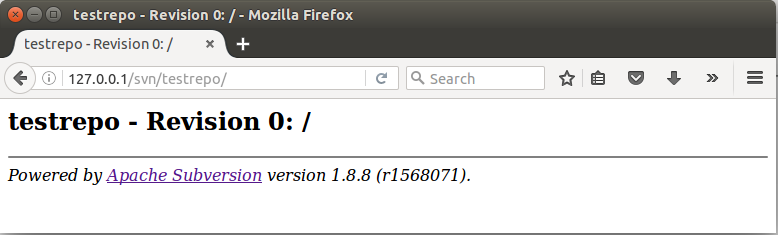
\includegraphics[scale=0.55]{./images/webtestrepo.png}
\end{center}
或者用 Subversion 客户端命令来检出工作副本:
\begin{center}
    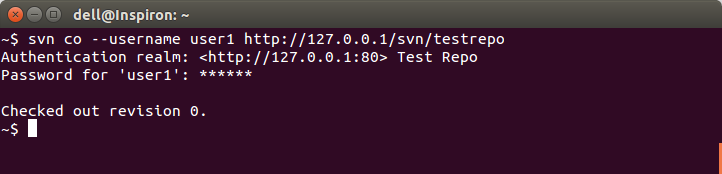
\includegraphics[scale=0.6]{./images/terminalrepo.png}
\end{center}

\backmatter
\pdfbookmark[0]{索引}{chap:index}
\printindex

\end{document}
